In order to successfully create patches in a requirements traceability environment, we must first understand the characteristics of the environment. To do this, we construct graphs of the environment following the Codebook paradigm. We then examine the types of human-human and human-artifact relationships that connect a traceability question to an identified answer; encoding these relationships can build a patch that a requirements traceability forager can explore to understand their prey\textemdash their need to understand their traceability question\textemdash better.

\section{The Information Environment}
\begin{table}[!b]
  \caption{Jira Projects and Characteristics}
  \centering
  \begin{tabular}{ |c|| c | c | c | c |  }
    \hline
    Project & Domain & Written & \makecell{Initial \& Latest\\Releases Examined} & \makecell{Questions} \\
    \hline
    \makecell{DASHBUILDER} & \makecell{data\\reports} & \makecell{Java,\\HTML} & \makecell{Aug 27, 2014 \& \\Apr 14, 2016} & 31 \\
    \hline
    DROOLS & \makecell{business\\rules} & Java & \makecell{Nov 13, 2012 \&\\Jul 17, 2017} & 57 \\
    \hline
    \makecell{IMMUTANT} & \makecell{complexity\\reduction} & Clojure & \makecell{Mar 14, 2012 \&\\Jun 23, 2017} & 18 \\
    \hline
    JBTM & \makecell{business\\process} & \makecell{Java,\\C++} & \makecell{Dec 5, 2005 \&\\Jul 14, 2017} & 5 \\
    \hline
  \end{tabular}
  \label{tab:jiraProjects}
\end{table}

\begin{table}[!t]
  \centering
  \small
  \caption{Select Questions with Identified Answers from DROOLS}
  \tabcolsep=0.11cm
  \scalebox{0.70}{
    \begin{tabular}{ |l|l|l|l|l|l|l|  }
      \hline
      id & issue & body & asker & answered by & role & operations \\
      \hline
      1206 & 972 & Can you please send a PR adding a new example...? \ldots & Mario Fusco & Mauricio Salatino & Creator & add pull request \\
      1220 & 963 & This should be fixed for 6.4.0.Final, does it sound possible? & Mauricio Salatino & Petr Siroky & Assignee & change fix version \\
      1371 & 907 & ...Please look at [my page]. What do you think\ldots & Michael Kiefer & Geoffrey De Smet & Creator & marked as done \\
      1377 & 905 & Thanks...[\textasciitilde martenscs]. Is there any other prefix?  \ldots & Petr Siroky & & & \\
      1383 & 901 & any news here [\textasciitilde mfusco]? & David naranjo & Geoffrey De Smet &  & provide opinion \\
      1627 & 823 & Hi Geoff, I don't know what shoud be the expected behaviour? \ldots & Michael Kiefer &  &  & \\  
      \hline
  \end{tabular}
  }
  \label{tab:drools}
\end{table}


% - Why Jira?
The literature suggests that issue trackers are essential for open-source projects to manage requirements~\cite{ICSE5,ICSE25,ICSE33,ICSE40,ICSE60}. Although the requirements of an open-source project can originate from emails, how-to guides, and other socially lightweight sources~\cite{ICSE62}, the to-be-implemented requirements ``eventually end up as feature requests in an issue-tracking system''~\cite{ICSE33}. We therefore turn to the issue-tracking system Jira, with issues like Figure \ref{fig:drools} to understand the life of requirements.

\begin{figure}
  \centering
  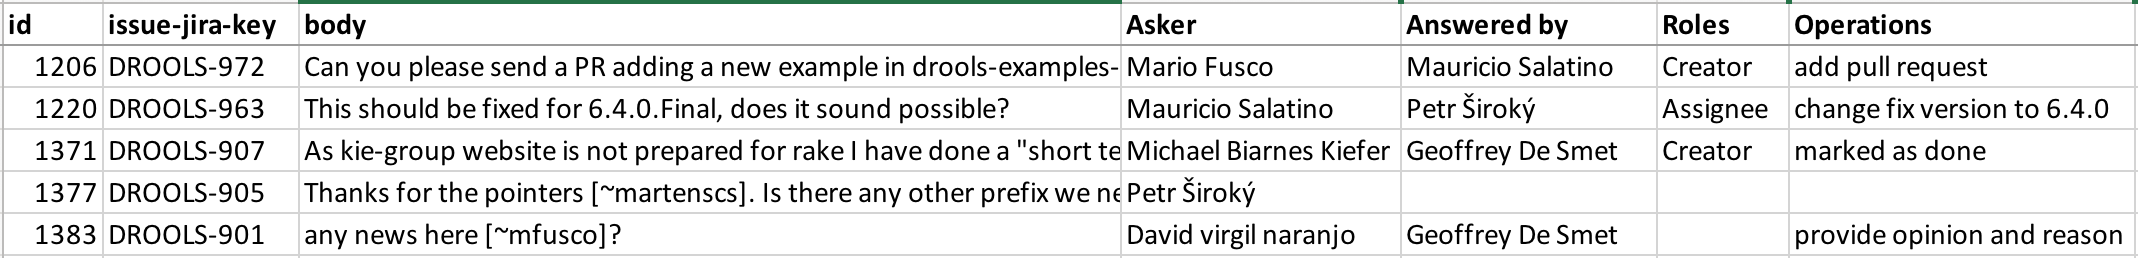
\includegraphics[width=\linewidth]{drools.png}
  \caption{A Screenshot of a Common Issue in Jira, in the DROOLS project. From this, we will take Issue, Assignee, Reporter/Creator, and questions like the first comment.}
  \label{fig:drools}
\end{figure}


% - Why 6 projects within Jira?
From Jira, we select four open-source projects from the Apache software foundation~\cite{ICSE7} or the JBoss family~\cite{ICSE38}.
The four projects tackle problems in different domains with implementations written in different programming languages, as seen in Table \ref{tab:jiraProjects}.

% - within projects, requirements manifest themselves as questions
Within the chosen projects, we focus on questions and answers. As discussed, questions represent a traceability forager's information need. By finding the exact person who answered a forager's question, we can gain insight into the information environment; we \textit{know} that the person who answered a traceability question can provide information on the traceability issue. For each project, two researchers identified comments that were questions (using tools from Stanford's CoreNLP project ~\cite{corenlp} to identify questions in multiple forms, e.g., with/without a question mark) and identified the respective answer comments, building their answer sets individually. Some examples of the answer sets generated can be seen in Table \ref{tab:drools}. The researchers reached a substantial degree of agreement (average Cohen's kappa=0.67) on requirements traceability questions over the 4 projects. Discrepancies were resolved in a joint meeting between the researchers. 

With our information environment identified, the next step to creating patches is to build a requirements socio-technical graph (RSTG) so that we can inspect the topology of the environment using graph theory concepts. A graph requires nodes and edges.

\section{Constructing Requirements Socio-Technical Graphs}
\subsection{Nodes}
% - why do we considered these projects heterogeneously? 
% - what are our node types? issues, comments, and people.
In Jira, issues (typically tasks or feature requests) are our requirements. Comments are provided to the issue, and may contain questions or answers. Users create issues, are assigned to issues, submit comments, and reference other users within their comments. This process can be seen in the screenshot of a typical Jira issue in Figure \ref{fig:drools}. Contemporary approaches to requirements traceability are either artifact-based (e.g., trace retrieval) and would consider only the comments and issues~\cite{ICSE15}, or are driven by social roles (e.g., contribution structures in the requirements specification production) and would consider the relationships of the people~\cite{ICSE29}. As we constructed our answer set, however, we realized the impact of the people-artifact relationships on the ability to track a requirement's life. Therefore, we consider Jira's issues, comments, \textit{and} people in our information environment. These will serve as our nodes. What, then, serve as our edges?

\subsection{Edges}

\begin{figure}
	\centering
	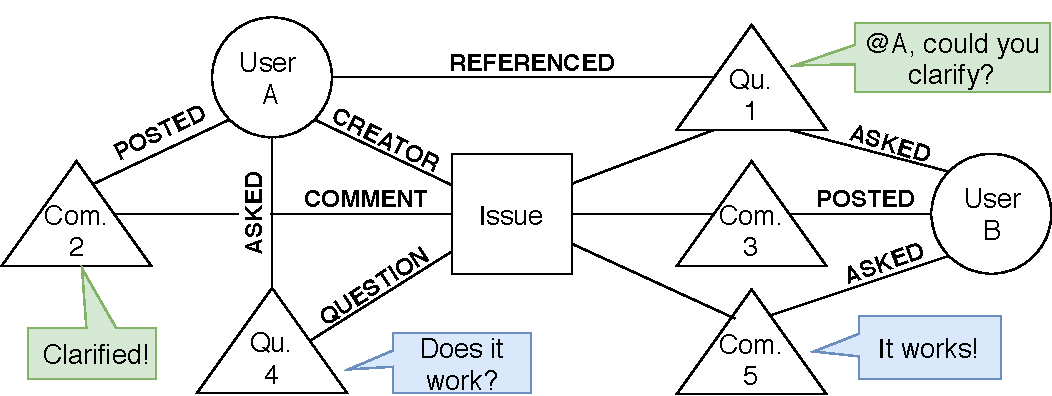
\includegraphics[width=\linewidth]{rstg.pdf}
	\caption{Requirements Socio-Technical Graph}
	\label{fig:rstg}
\end{figure}

By manually inspecting the paths between questions and their eventual answers, we are able to define the edges in our network topology. Consider the following example: Figure \ref{fig:rstg} is a subgraph from the IMMUNANT project, showing two questions and their answers. User 2881 created Issue 73650. User 6655, the forager, commented on the issue (Comment 149789), asking User 2881 for clarification by referencing them in the comment. User 2881 commented on the issue (Comment 149790), providing the clarification. In another foraging interaction, User 2881, now the forager, commented on the issue (Comment 149792), asking ``This is now available in [incremental build | http://immutant.org/builds/2x/] 591 and newer. Can you give that a try and confirm it works for you?'' User 6655 responded (Comment 149793) ``I've finally found the time to test this and can confirm it works! Thanks!''. 

These two foraging interactions demonstrate most of the relationships that we observed between nodes in the datasets. These relationships are treated as the edges within our graph:
\begin{samepage}
\begin{itemize}
  \item \textit{Creator:} Users create issues
  \item \textit{Commented, Asked: }Users post comments and questions
  \item \textit{Comment, Question:} Comments and questions are posted to Issues
  \item \textit{Referenced:} Comments can reference other users
  \item \textit{Assignee:} (Not pictured) Users can also be designated assignees on issues 
\end{itemize}
\end{samepage}
While some relationships could be considered as unidirectional, e.g., a user posting a comment, the comment also serves as a bridge connecting the issue to the user, who is knowledgeable on the issue. We therefore elected to encode the network as an undirected graph.

\subsection{Scripting Graph Construction}
With our desired node and edge types identified, we then automated graph construction in Python, leveraging the graph construction and analysis library, NetworkX ~\cite{networkx}, heavily. The full code described here can be found in our online repository ~\cite{repo}, as well as in Appendix \ref{app:python}. Our objective was to automate the construction of RSTGs like Figure \ref{fig:rstg} for each question, representing the state of the project at the time of the question. Representing the network at the time of the question was important to us so that only relationships that had existed prior to asking of the question would be considered.

In order to construct RSTGs, our script queried a database that held tables with the following characteristics. Note that irrelevant tables have been omitted:
\begin{itemize}
  \item \textit{jira\textunderscore issue:} All projects' issues, as well as assignee, creator, and a description
  \item \textit{jira\textunderscore issue\textunderscore comment:} All comments, as well as who posted them on which issue
  \item \textit{jira\textunderscore issue\textunderscore type:} Issue types, e.g., ``Bug'', ``New Feature'', ``Improvement''
  \item \textit{jira\textunderscore project:} Keys of projects in database, as well as names and descriptions. 
  \item \textit{jira\textunderscore user:} All of users' usernames, real names, and database IDs
\end{itemize}

We began by pulling all of a project's issues and associated users and adding them to a graph (\texttt{dbManager.addProjectIssuesToGraph(project,graph)}). This was performed by querying the database (\textsc{select * from jira\textunderscore issue where project = x}) and adding a node for each result, each result's creator, and each result's assignee. The creators and assignees were connected to their issue with a labeled edge.

Next, each comment was added to the graph, and was connected to its issue, author, and any referenced user (\texttt{dbManager.addProjectCommentsToGraph(project,graph)}) with the query \textsc{select * from jira\textunderscore issue\textunderscore comment where issue in ( select id from jira\textunderscore issue where project = x )}. While each issue has its creator and assignee explicitly defined by Jira, and each comment has its author and issue, some additional processing was required to identify references. In practice, a reference can either be the user's username (e.g., [\textasciitilde ge0ffrey]) or first name (e.g., ``Geoffrey,'' or ``Geoffrey:''). With regular expressions (\texttt{\textbackslash {[}\textasciitilde (.+?)\textbackslash {]}}), usernames were identified in the body of a comment and connected the comment to the user. However, a dictionary of first-name references had to be manually built so that an identified reference (regex: \texttt{{[}A-Z{]}{[}a-z{]}+?,|{[}A-Z{]}{[}a-z{]}+?:}) could be connected to its user. 

\section{Properties of Requirements Socio-Technical Graphs in Information Foraging}
We now tie our RSTGs to information foraging theory. When a forager asks a question, like the ones in Figure \ref{fig:rstg}, where do they find their answer? The location of the answer might grant us insight on what we should include in a patch of information relevant to a question. What path might the traceability forager typically follow to the user who will provide the answer, gathering information on their prey along the way?

\begin{figure}
	\centering
	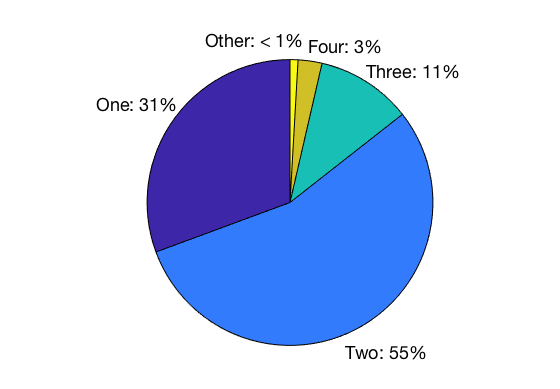
\includegraphics[width=\linewidth]{pie.png}
	\caption{Degrees of Separation between Question and Answer in Projects}
	\label{fig:pie}
\end{figure}

By analyzing the paths connecting question nodes and answer nodes, we identified recurring patterns connecting traceability questions with answers. The patterns are organized by degrees of socio-technical separation, which we define as the minimum number of edges to be traversed between two nodes. Figure \ref{fig:pie} displays the frequency of degrees separating questions and answers for our 125 questions. 

\subsection{One or Two Degrees of Separation From Question}
Figure \ref{fig:pie} shows that more than three-quarters of answers are within two degrees of the question. These represent simple foraging tasks. By the time a forager posts a question, they may be relatively familiar with an issue. The very fact that they chose a specific issue to comment on demonstrates that they expect their answer to be near the issue. A well-informed forager will often reference the exact user they expect to know the answer. These kinds of relationships fall within this category.

\begin{figure}[ht]
	\centering
	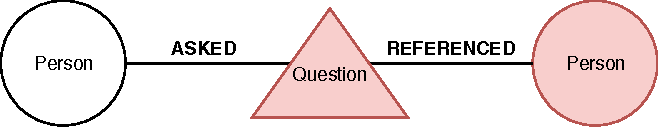
\includegraphics[width=\linewidth]{1deg.pdf}
	\caption{Referenced (1 Degree)}
	\label{fig:1deg}
\end{figure}

Within one degree of the question, two types of answers were observed. The first is when the forager answers their own query. Because the forager, in the RSTG, is directly connected to their comment, this is one degree of separation. The second is when a user is referenced within a comment. As shown in Figure \ref{fig:1deg}, when a user is referenced in a comment, they are directly connected to the comment. Comment 70842, from the DROOLS project, is a good example of this: "What should the URL look like in your opinion [\textasciitilde tirelli]?" asks User 4079. User tirelli answers. A vast majority of the 31\% of answers one degree away from the question came from direct references.

\begin{figure}[ht]
	\centering
	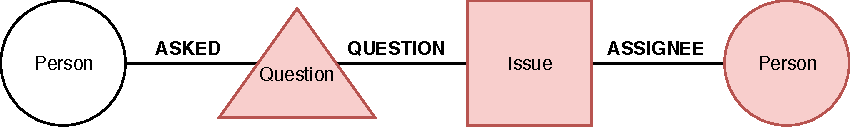
\includegraphics[width=\linewidth]{2deg.pdf}
	\caption{Creator or Assignee (2 Degrees)}
	\label{fig:2deg}
\end{figure}

Within two degrees of separation, we observed two more types of answers: when a forager asks a question on an issue, either the issue creator or issue assignee often responds. Figure \ref{fig:2deg} shows this interaction. When a forager posts a question to an issue without a reference, the creator, with their knowledge of what the issue is, or the assignee, with knowledge of what is being done to solve the issue, can answer. In Comment 353748, from the JBTM project, User 133 posts to an issue: ``Status update please?'' User 3619, assignee, provides an answer.

\subsection{Collaborators and Contributors\textemdash Three or Four Degrees of Separation From Question}
More challenging foraging occurs when the user with the answer is three or more degrees of separation away from the question. With each degree, the number of information artifacts and other users a forager must traverse increases exponentially. Identifying patterns and presenting useful patches to the forager in this class of foraging presents far greater potential. We present a few of the most frequent types of interactions that occur within this radius. 

\begin{figure}[ht]
	\centering
	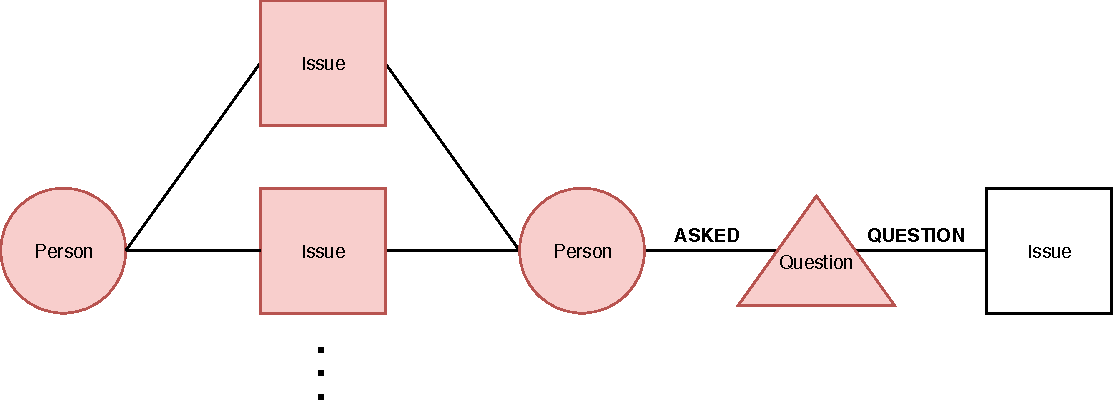
\includegraphics[width=\linewidth]{3degCollab.pdf}
	\caption{Frequent Collaborator of Asker or Referenced User (3 Degrees)}
	\label{fig:3degCollab}
\end{figure}

Most answers in our projects within three degrees of separation were of the type shown in Figure \ref{fig:3degCollab}: Comment--Person--Issue--Person. The question connects to a person\textemdash either the traceability forager or a referenced user\textemdash and the answer comes from a \textit{Frequent Collaborator}. While neither the forager themselves nor a referenced user has an answer, someone they collaborate with does. The Collaborator is connected with the user or the referenced by one or more comments (where the Collaborator is directly referenced). We notice that Collaborators are often highly-central users in a project, whose Frequent Collaborator status arises from their frequent contributions to projects. In other words, they are Frequent Collaborators because they are frequent users in general.

\begin{figure}[ht]
	\centering
	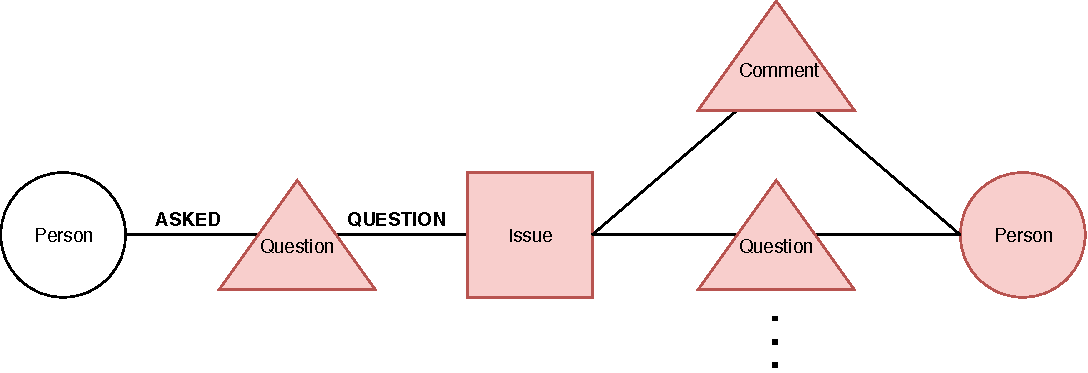
\includegraphics[width=\linewidth]{3degContrib.pdf}
	\caption{Frequent Contributor to Issue (3 Degrees)}
	\label{fig:3degContrib}
\end{figure}

The second type of answer within three degrees of separation is that shown in Figure \ref{fig:3degContrib}: Comment--Issue--Comment--Person. We call this type of answer a \textit{Frequent Contributor}. This user does not directly know the forager, nor are they creator or assignee of the issue. However, the Contributor has commented and asked on a given issue one or more times. Again, Frequent Contributors tend to be highly-central users. Figure \ref{fig:pie} shows that Frequent Collaborators and Frequent Contributors represent 11\% of answers in our dataset.

\begin{figure}[ht]
	\centering
	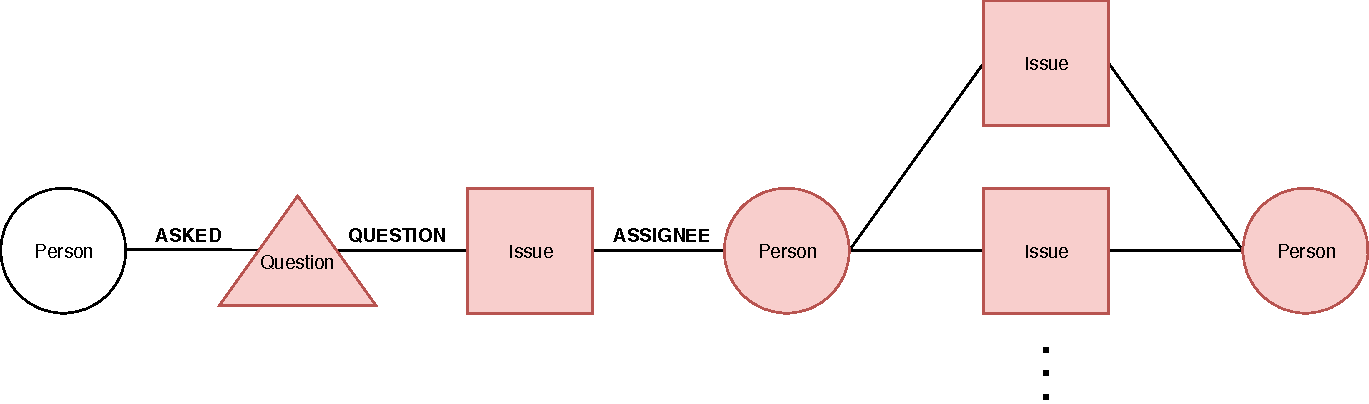
\includegraphics[width=\linewidth]{4degCollab.pdf}
	\caption{Frequent Collaborator of Creator or Assignee (4 Degrees)}
	\label{fig:4degContrib}
\end{figure}

Within four degrees, we see another variant of The Collaborator: a \textit{Frequent Collaborator of the Creator or Assignee} (Figure \ref{fig:4degContrib}). This type of relationship is signified by the pattern Comment--Issue--Person--Issue--Person. The creator or assignee of the issue has collaborated with the answerer on other issues before, either as creator or assignee on those issues. While the creator or assignee of the primary issue being considered may not have the answer, someone they often work with may. Figure \ref{fig:pie} shows that these kinds of interactions represent 3\% of our dataset.

We hypothesize that, within three or four degrees of separation, several other types of collaborators could be observed. Frequent Collaborators of the Asker could manifest by Comment--Person--Comment--Person, rather than Comment--Person--Issue--Person as we observed. Within four degrees, we observed Frequent Collaborators of Creators or Assignees; a Frequent Collaborator of the Asker could also show up within four degrees (Comment--Person--Issue--Comment--Person, or Comment--Person--Comment--Issue--Person). 


\subsection{Five or More Degrees of Separation}
In our sample set of 125 questions, there were no instances of five or more degrees of separation. Within this class, though, we hypothesize that more interesting variations of Frequent Collaborators and Frequent Contributors would arise; if one user does not know the answer, someone they know will. However, not having observed this class, we do not anticipate that it will be a commonplace sight.

\subsection{Unconnected Users}
\label{unconnectedusers}
\begin{figure}[ht]
	\centering
	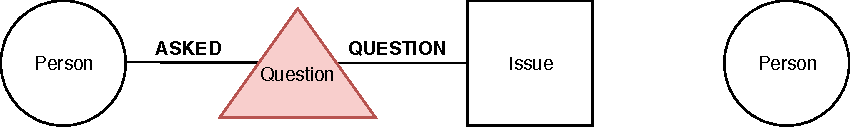
\includegraphics[width=\linewidth]{disconnected.pdf}
	\caption{Answer disconnected from network}
	\label{fig:disconnected}
\end{figure}

The final pattern observed was one instance of an answer unconnected from the graph of the project (Figure \ref{fig:disconnected}). At the time the question was asked, the user who will eventually answer the forager's traceability question was not yet connected to the project by the relationships we chose to express as edges. (For example, in Appendix \ref{app:cytoscape}, Figure \ref{fig:c9396}, some users are not in the network at the time of that comment). When that user finally did connect to the the network, they were four degrees of separation away (Comment--Person--Comment--Issue--Person), appearing as the assignee to an issue where the asker had commented. With a larger dataset, these not-yet-connected relationships would be interesting to assess. More edge and node types could enable a connection between that user and the question.

\begin{table}[!ht]
	\caption{Number of Nodes Within N Degrees of Question}
	\centering
		\begin{tabular}{ |c||c|c|c|c|c|  }
		\hline
		& Min & Q1 & Med & Q3 & Max \\
		\hline
		2 Degrees & 4 & 29   & 192  & 442  & 1908 \\
		3 Degrees & 5 & 271  & 510  & 1405 & 4192 \\
		4 Degrees & 5 & 625  & 2288 & 3636 & 7542 \\
		5 Degrees & 5 & 1949 & 3084 & 4597 & 7950 \\
		\hline
	\end{tabular}
	\label{tab:radiusStats}
\end{table}

It appears, from these classes, that a substantial amount of traceability foraging takes place in four-or-less degrees of separation. Seeking to apply information foraging to traceability, one could simply present all nodes within three-to-four degrees of the question as a patch where the forager might seek to understand their question. This would satisfy our requirement of encoding frequently-traversed foraging paths into a patch. However, as shown in Table \ref{tab:radiusStats}, these patches are extremely large. If we included all nodes within 4 degrees of separation, most patches would have over 2200 nodes. Appendix \ref{app:cytoscape}, Figures \ref{fig:degpatch2}, \ref{fig:degpatch3}, and \ref{fig:degpatch4} may emphasize this further: thanks to a central user, foraging through these patches seems entirely impractical. With some notion of relatedness, however, these patches could be made smaller without losing relevant information.